\documentclass{beamer}
\usetheme{Frankfurt}
 
\usepackage{multicol}
\usepackage{bm}
\usepackage{amssymb}                            % (1)
\usepackage{amsthm}                             % (2)
\usepackage{graphicx}                           % (3)
\usepackage{xmpmulti}
\usepackage[none]{hyphenat}
\usepackage{bm}
\usepackage{amsmath}
\usepackage{tabu}
\usepackage{comment}
\usepackage{enumitem}
\usepackage[ruled,vlined]{algorithm2e}
\usepackage{graphicx}
\usepackage{setspace}
\usepackage{caption}
\usepackage{subcaption}

\usepackage{float}
\usepackage{alltt}


\title{Functional Principal Component Analysis for Manifold Data}
\date{\today}


\begin{document}

\maketitle
\section{Introduction}
\subsection{Manifolds}

\begin{frame}{Types of manifolds or manifolds with additional structures}
\begin{itemize}
  \item $\bullet$ Topological Manifold:  spheres are same as cubes.
  \item $\bullet$ Differential Manifold: spheres and ellipsoids are same.
  \item $\bullet$ Riemannian Manifold: equipped with Riemannian metric for defining angles and distances.
  \end{itemize}
\end{frame}


\begin{frame}{Example: manifolds}
\begin{figure}
\centering
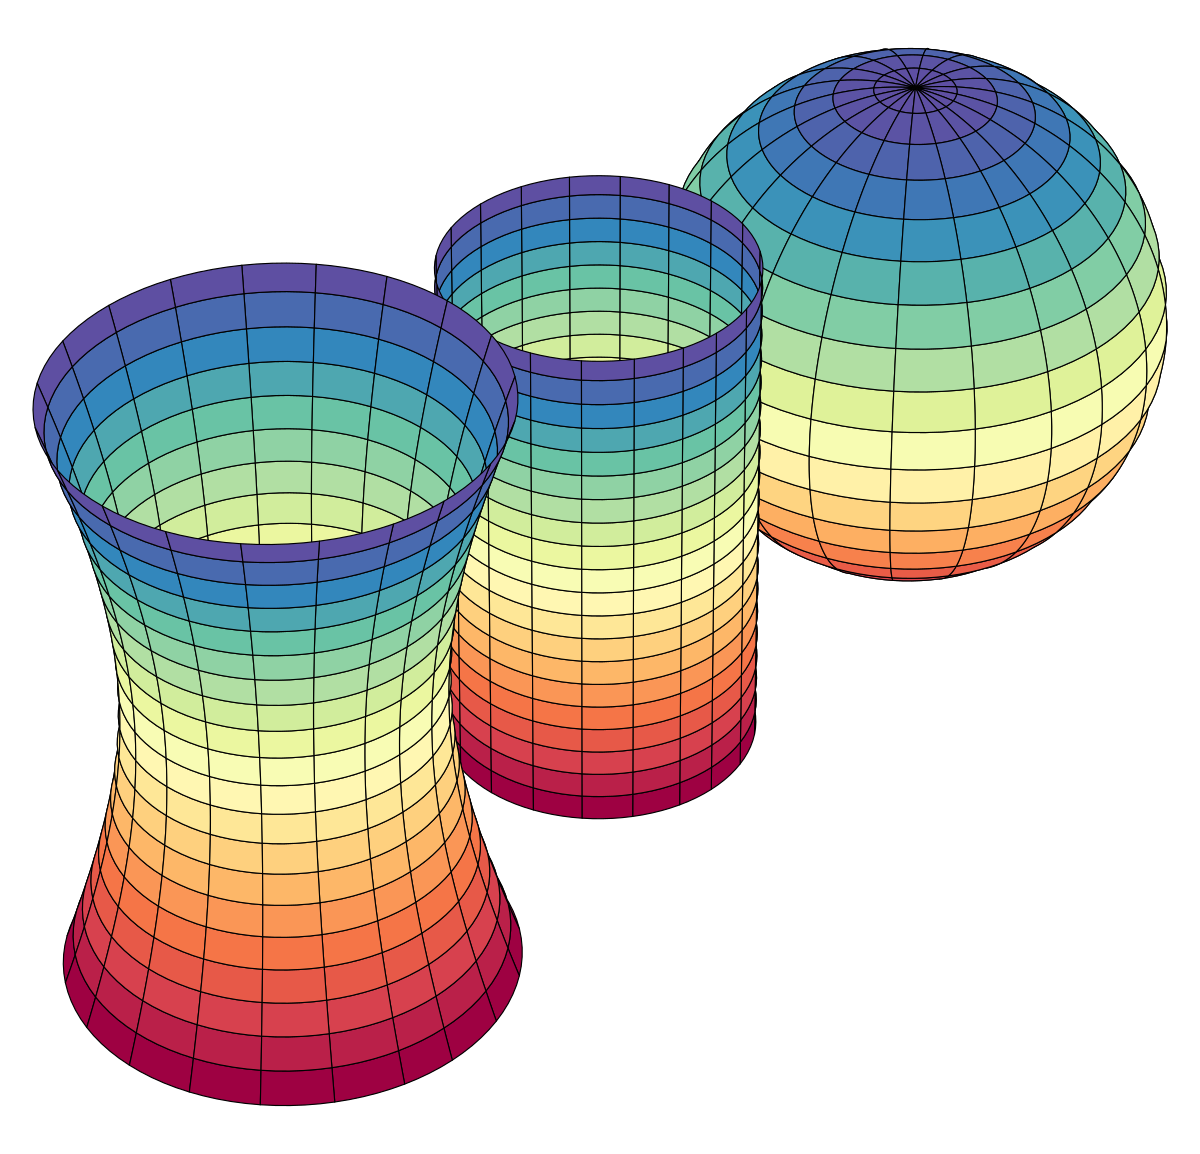
\includegraphics[scale=0.2]{manifoldexample.png}
\end{figure}
\end{frame}

\begin{frame}{Example: n-sphere}
The n-sphere $\mathbb{S}^{n}$ is an n-dimensional manifold that can be embedded in Euclidean (n + 1)-space.
\begin{equation*}
  \mathbb{S}^{n} = \{x \in \mathbb{R}^{n+1}: ||x|| = r\}
\end{equation*}
\begin{itemize}
  \item A pair of points on the real line is 0-sphere.
  \item A circle on $\mathbb{R}^{2}$ is 1-sphere.
  \item Surface of a ball is 2-sphere.
  \end{itemize}
\end{frame}

\begin{frame}{Manifolds}
\begin{alertblock}{Importance}
Manifolds locally resemble Euclidean space near each point, i.e., point of n-manifold has a neighbourhood that is homeomorphic to the Euclidean space of dimension n.
\end{alertblock}
\end{frame}

\begin{frame}{Example 1}
\begin{figure}
\centering
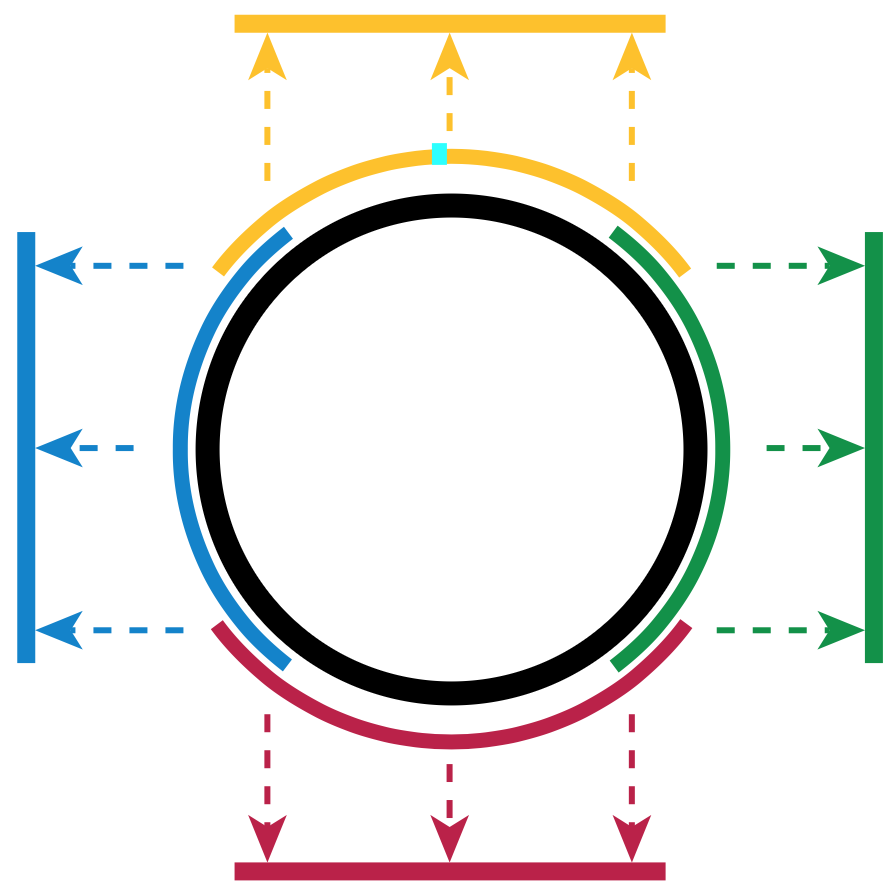
\includegraphics[scale=0.5]{chart-circle.png}
\end{figure}
\end{frame}

\begin{frame}{Example 2}
\begin{figure}
\centering
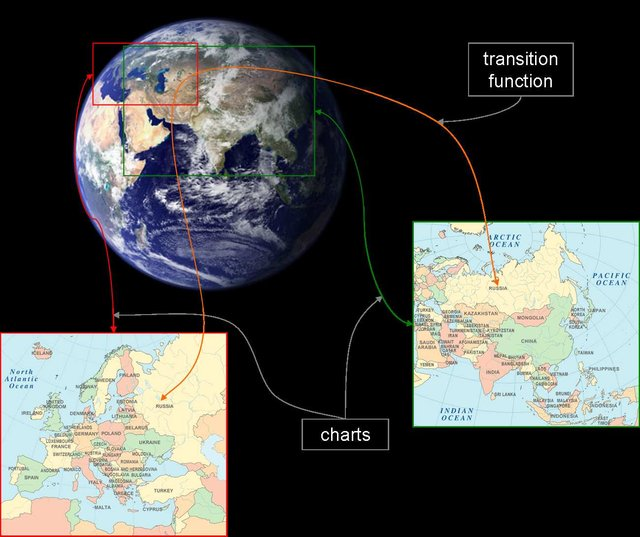
\includegraphics[scale=0.4]{charts-globe.jpg}
\end{figure}
\end{frame}

\subsection{Geodesics}
\begin{frame}{Geodesics}
\begin{alertblock}{Geodesics: generalization of straight lines}
\begin{itemize}
  \item $\bullet$ Like straight lines in Euclidean spaces, we need a `straight line' to quantify distance.
  \item $\bullet$ Geodesics are the curves on a smooth manifold that locally yield the shortest distance between two points.
  \end{itemize}
  \end{alertblock}
\end{frame}

\begin{frame}{Geodesics: example}
\begin{figure}
\centering
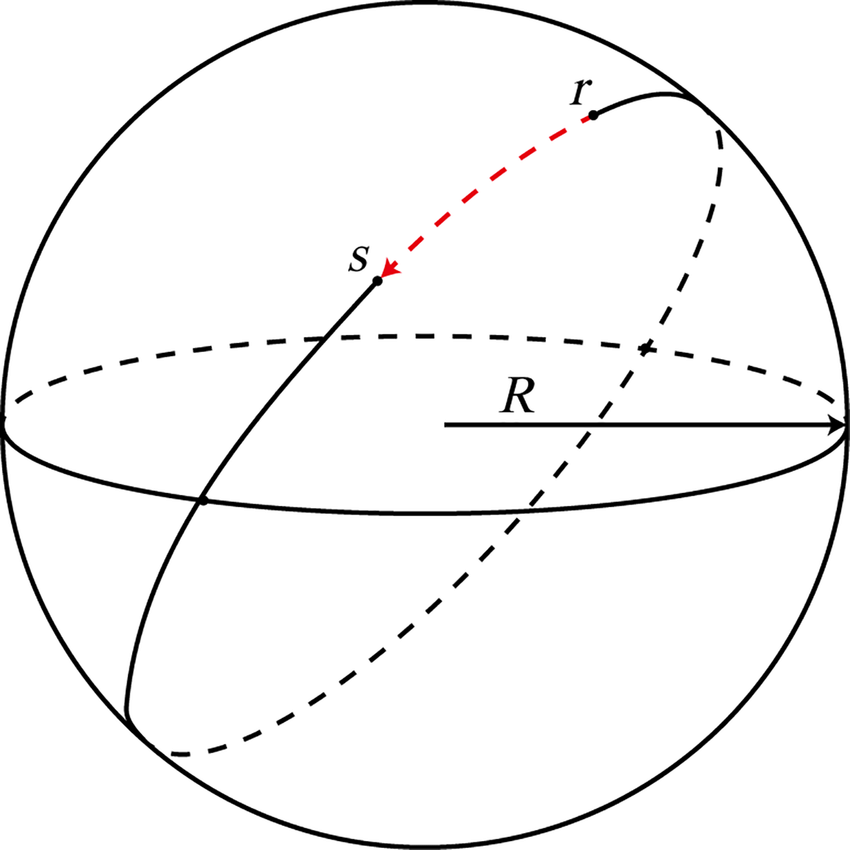
\includegraphics[scale=0.2]{great_circle.png}
\end{figure}
\end{frame}

\begin{frame}{Geodesic distance}
	\begin{figure}
		\centering
		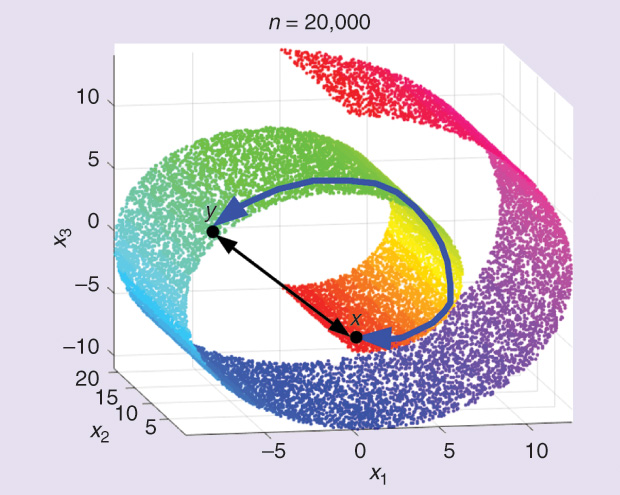
\includegraphics[width=\textwidth]{geodesicdistance.jpg}
    \end{figure}
\end{frame}


\subsection{Tangent space}
\begin{frame}{Tangent space $T_{p}M$}
\begin{itemize}
   \item $\bullet$ A tangent space $T_{p}M$ is a real vector space containing all vectors passing a point $p$ on a n-manifold $M$.
   \item $\bullet$ $T_{p}M$ is also n-dimensional and same as the manifold $M$.
   \item $\bullet$ Tagent space provides the best linear approximation to the manifold around $p$ (Taylor expansion).
\end{itemize}
\end{frame}


\begin{frame}{Tangent space: Example}
\begin{figure}
\centering
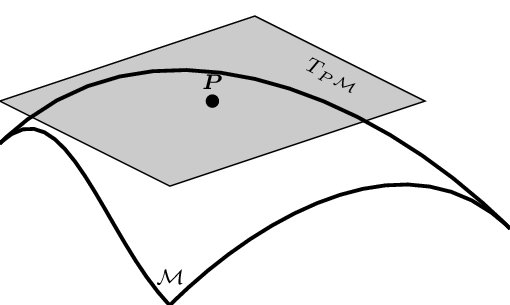
\includegraphics[width=\textwidth]{tangent_space.jpg}
\end{figure}
\end{frame}

\begin{frame}{Tangent space: Linear approximation}
Assume we have a 2-dimensional manifold parametrized as $z = f(x,y)$. Taking the Taylor expansion
\begin{equation*}
 z = f(x,y) \approx f(p) + \nabla f(p) \dot ((x,y) - p) + \cdots
\end{equation*}
which gives the tangent space or plane.
\end{frame}

\subsection{Mapping}
\begin{frame}{Exponential map}
Let $\mathcal{D}(p)$ be an open subset of $T_{p}M$ defined by
\begin{equation*}
\mathcal{D}(p) = \{ v \in T_{p}M | \gamma_{v}(1) \text{ is defined}\}
\end{equation*}
where $\gamma_{v}$ is the unique geodesic with $\gamma_{v}(0) = p$ and $\gamma^{\prime}_{v}(0) = v$.
\begin{alertblock}{{\color{blue} Exponential map}}
\begin{equation*}
  \text{exp}_{p}(v):\mathcal{D}(p) \rightarrow M \text{, given by } \text{exp}_{p}(v) = \gamma_{v}(1)
\end{equation*}
\end{alertblock}
\end{frame}

\begin{frame}{Exponential map}
\begin{itemize}
  \item $\bullet$ Local parametrization of the manifold $M$.
  \item $\bullet$ A map from the subspace of $T_{p}M$ to $M$.
  \item $\bullet$
  \begin{figure}
  \centering
  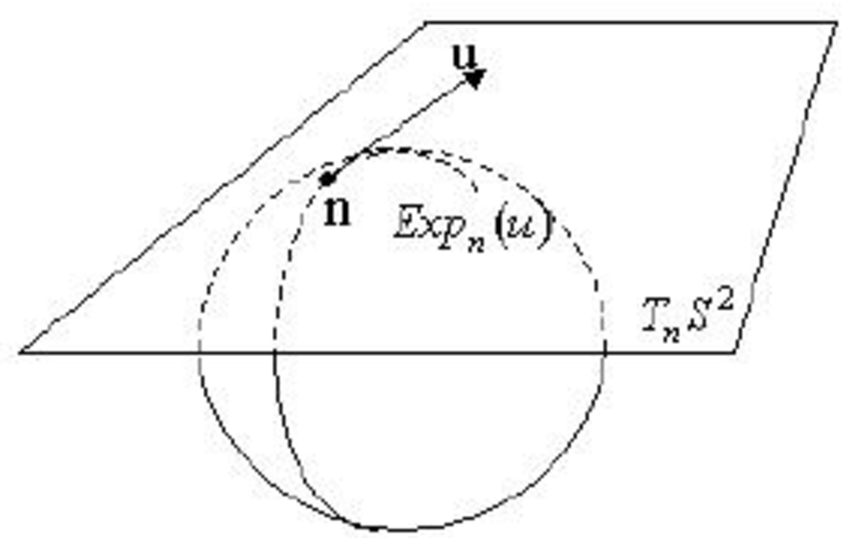
\includegraphics[scale=0.2]{The-exponential-map.png}
  \end{figure}
\end{itemize}
\end{frame}

\begin{frame}{Radius of injectivity}
\begin{alertblock}{Injectivity radius $\text{inj}_{p}$}
   Let $M$ be a smooth manifold. $\forall p \in M$, the {\color{blue} injectivity radius} of $M$ at $p$ is the supremum such that $\text{exp}_{p}$ is a diffeomorphism on the open ball $B(0,r) \subseteq T_{p}M$.
  \end{alertblock}
  Diffeomorphism means that there is a smooth inverse function of $\text{exp}_{p}$ which is the logarithm map $\text{log}_{p}$.
\end{frame}
\begin{frame}{example}
\begin{figure}
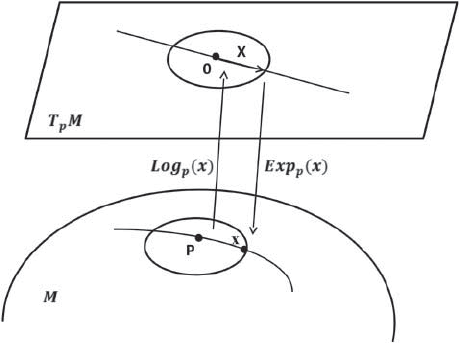
\includegraphics[scale = 0.5]{logmap.png}
\end{figure}
\end{frame}



\begin{frame}{Sphere example}
The geodesic distance between any points $p_{1}$ and $p_{2}$ on a sphere is the great-circle distance,
\begin{equation*}
  d_{M}(p_{1},p_{2}) = \text{cos}^{-1}(p_{1}^{T}p_{2})
\end{equation*}
The exponential map given a point $p$ on the manifold is 
\begin{equation*}
  \text{exp}_{p}(\bm{v}) = \text{cos}(||\bm{v}||_{E})p + \text{sin}(||\bm{v}||_{E})\frac{\bm{v}}{||\bm{v}||_{e}}
\end{equation*}
The logrithm map $\text{log}_{p}:M \setminus\{-p\} \rightarrow T_{p}M$ is the inverse of the exponential map 
\begin{equation*}
  \text{log}_{p}(q) = \frac{q-(p^{T}q)p}{||q-(p^{T}q)p||}d_{M}(p,q)
\end{equation*}
\end{frame}



\section{FPCA for data on manifold}
\subsection{Preliminaries}
\begin{frame}{Notations}
Let $\mathcal{M}$ be a d-dimensional complete Riemannian manifold embedded in a Euclidean space $\mathbb{R}^{d_{0}}$ for $d \leq d_{0}$. $\mathcal{X}$ denotes the sample space of  $\mathcal{M}$-valued function where
\begin{equation*}
\mathcal{X} = \{x : \mathcal{T} \rightarrow \mathcal{M} | x \in C(\mathcal{T})\}
\end{equation*}
for some compact interval $C(\mathcal{T}) \subset \mathbb{R}$.
\end{frame}


\begin{frame}{Frechet mean}
Like variables in Euclidean space, we need to define the mean or the expectation for the $\mathcal{M}$-valued function $X(t)$. The Frechet mean is introduced as the global minimizer of the aggregate energy function or the sum of squared distance for each $t \in \mathcal{T}$. That is,
\begin{equation*}
M(p,t) = \sum_{j=1}^{J}d^{2}_{\mathcal{M}}(X_{j}(t),p) \text{ and } \mu_{\mathcal{M}}(t) = \underset{p\in\mathcal{M}}{\text{argmin}M(p,t)}
\end{equation*}
\end{frame}

\begin{frame}{Idea of RFPCA}
The idea of RFPCA is to represent the variation of the inifite dimensional object $X$ around the mean function $\mu_{\mathcal{M}}$ in a lower dimensional submanifold.
\end{frame}

\begin{frame}{Basis expansion}
The K-dimensional submanifold is defined in the following way
\begin{itemize}
  \item $\bullet$ Given a system of K orthonomral basis functions $\psi_{k}(t) \in T_{\mu_{\mathcal{M}(t)}}$.
  \item $\bullet$ The submanifold
  \begin{equation*}
  \mathcal{M}_{K}(\bm{\Psi}_{K}):= \{x\in\mathcal{X},x(t) = \text{exp}_{\mu_{M}(t)}(\sum_{k=1}^{K}a_{k}\psi_{k}(t))| t\in\mathcal{T},a_{k}\in\mathbb{R}\}
  \end{equation*}
\end{itemize}
\end{frame}


\begin{frame}{The best K-dimensional approximation to X}
Let $\Pi(x,\mathcal{M}_{K})$ be the projection of $x\in\mathcal{X}$ on $\mathcal{M}_{K}$ which is defined as
\begin{equation*}
       \Pi(x,\mathcal{M}_{K}):= \underset{y\in\mathcal{M}_{K}}{\text{argmin}}\int_{\mathcal{T}}d_{\mathcal{M}}(y(t),x(t))^{2}dt
\end{equation*}
The best K-dimensional approximation to X is then find a submanifold $\mathcal{M}_{K}$ that minimizes
\begin{equation*}
F_{S}(\mathcal{M}_{K}) = E\int_{\mathcal{T}}d_{\mathcal{M}}(X(t),\Pi(X,\mathcal{M}_{K})(t))^{2}dt
\end{equation*}
where each manifold is generated by K basis functions.
\end{frame}

\begin{frame}{Logarith mapping}
Instead of directly optimizing $F_{S}(\mathcal{M}_{K})$ over a family of manifolds, the objective function is modifed by invoking tangent space approximation. Recalling injectivity radius and exponential map with its inverse logarithm map,
\begin{equation*}
V(t) = log_{\mu_{\mathcal{M}}(t)}(X(t))
\end{equation*}
is well-defined for all $t\in\mathcal{T}$ as long as $X(t)$ stays within $\text{inj}_{\mu_{\mathcal{M}}(t)}$.

\end{frame}

\begin{frame}{Optimization}
A practical and tractable optimality criterion is therefore defined as
\begin{equation*}
    F_{V}(\mathcal{V}_{K}) = E(||V - \Pi(V,\mathcal{V}_{K})  ||^{2})
\end{equation*}
over all K-dimensional linear subspaces
\begin{equation*}
 \mathcal{V}_{K}(\psi_{1},...,\psi_{K}) = \{\sum_{k=1}^{K}a_{k}\psi_{k}(t)|a_{k}\in\mathbb{R}\}
\end{equation*}
for $\psi_{k} \in \mathbb{H}$ and $\psi_{k}(t) \in T_{\mu_{\mathcal{M}(t)}}$. This is equivalent to a multivartiate functional principal component analysis.
\end{frame}

\begin{frame}{Covariance $G(t,s)$ ov $V(t)$}
Let $G(t,s)$ be the covariance function of $V(t)$ in $L^{2}$ sense. Then,
\begin{equation*}
G(t,s) = cov(V(t),V(s)) = E(V(t)V(s)^{T})
\end{equation*}
since the log-mapped data $V(t) = log_{\mu_{\mathcal{M}}(t)}(X(t))$ is zero at the intrinsic mean of data on manifold.
\end{frame}

\begin{frame}{Karhunen-Loeve decomposition of $V(t)$}
Let
\begin{equation*}
G(t,s) = \sum_{k=}^{\infty} \lambda_{k}\phi_{k}(t)\phi_{k}(s)^{T}
\end{equation*}
where $\phi_{k}$'s are the orthonormal vector-valued eigenfucntions with eigenvalues $\lambda_{k}$. Then, the Karhunen-Loeve decomposition of $V(t)$ is
\begin{equation*}
V(t) = \sum_{k=1}^{\infty} \xi_{k}\phi_{k}(t)
\end{equation*}
where $\xi_{k} = \int_{\mathcal{T}}V(t)\phi_{k}(t)dt$ is the k-th RFPC score.
\end{frame}


\begin{frame}{Best K-dimensional approximation}
The Best K-dimensional approximation to $V$ is $V_{k}$ that minimizes
\begin{equation*}
E(||V - \Pi(V,\mathcal{V}_{K})  ||^{2})
\end{equation*}
\end{frame}

\begin{frame}{Illustration}
\begin{figure}
\centering
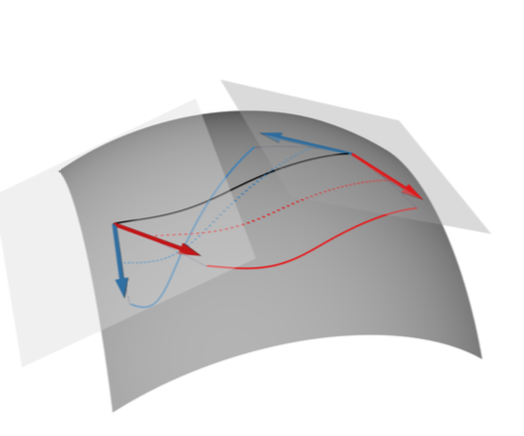
\includegraphics[scale=1]{karhunen.png}
\end{figure}
\end{frame}


\begin{frame}{Choosing a suitable $K$}
When $K = 0$, $V_{0}(t) = 0$ and $X_{0}(t) = \mu_{\mathcal{M}}(t)$. Define $U_{K}$ to be the residual variance as
\begin{equation*}
U_{K} = E\int_{\mathcal{T}}d_{\mathcal{M}}(X(t),X_{K}(t))^2dt
\end{equation*}
The fraction of varinance explained by the first K components as
\begin{equation*}
\text{FVE}_{K} = \frac{U_{0} - U_{k}}{U_{0}}
\end{equation*}
$K^{\star}$ is chosen as the smallest K with largest FVE.
\end{frame}

\subsection{Estimation procedure}

\begin{frame}{Estimation I}
Given a Riemannian manifold $\mathcal{M}$ with n independent observations $X_{1},...,X_{n}$, which are $\mathcal{M}$-valued random functions that are distributed as X.
\begin{itemize}
  \item $\bullet$ Sample Frechet mean $\hat{\mu}_{\mathcal{M}}(t)$ is obtained by minimizing $M_{n}(p,t) = \frac{1}{n}\sum_{i=1}^{n}d_{\mathcal{M}}(X_{i}(t),p)^{2}$.
  \item $\bullet$ The log-mapped data $V_{i}$: $\hat{V}_{i}(t) =\text{log}_{\hat{\mu}_{\mathcal{M}}(t)}(X_{i}(t))$.
  \item $\bullet$ Sample covariance function $\hat{G}(t,s) = \frac{1}{n}\sum_{i=1}^{n}\hat{V}_{i}(t)\hat{V}_{i}(s)$
\end{itemize}
\end{frame}

\begin{frame}{Estimation II}
\begin{itemize}
  \item $\bullet$ Obtain k-th eigenvalue and eigenfunction $(\hat{\lambda}_{k},\hat{\phi}_{k})$ of $\hat{G}$.
  \item $\bullet$ Calculate kth RFPC score of each subject $\xi_{ik} = \int_{\mathcal{T}}V_{i}(t)\phi_{k}(t)dt$.
  \end{itemize}
  Hence, the K-dimensional representation becomes
  \begin{equation*}
    \hat{V}_{iK}(t) = \sum_{k=1}^{K}\hat{\xi}_{ik}\hat{\phi}_{k}(t) , \hat{X}_{iK}(t) = \text{exp}_{\hat{\mu}_{\mathcal{M}(t)}}(\sum_{k=1}^{K}\hat{\xi}_{ik}\hat{\phi}_{k}(t))
  \end{equation*}
\end{frame}


\section{Example}
\begin{frame}{Example: Vancouver wind data}
\end{frame}

\begin{frame}{Finding Frechet mean}
\begin{equation*}
M(p,t) = \sum_{j=1}^{J}d^{2}_{\mathcal{M}}(X_{j}(t),p) \text{ and } \mu_{\mathcal{M}}(t) = \underset{p\in\mathcal{M}}{\text{argmin}M(p,t)}
\end{equation*}
The above can be thought of as a function of angles, and we can develope a naive gradient descent to search for the minimizer given the uniqueness in 1-sphere case. 
\begin{equation*}
  p^{(i+1)} = p^{(i)} - \frac{dM(p,t)}{dp^{(i)}}
\end{equation*}
\end{frame}

\begin{frame}{}
 \centering \Huge
  \emph{Go to R...}
\end{frame}


\begin{frame}{}
  \centering \Huge
  \emph{Thank You}
\end{frame}



\end{document}